\section{Multi-Level Clock}\label{sec:multiLevelClock}

\subsection{Preliminaries}

A clock that can measure only two times in one cycle of a periodic evolution
is of limited interest ---and limited falsifiability, as it can be easily
interpolated by different models.
The experiment described in
\cite{Moreva:synthetic} and related works attempts at addressing the issue:
\begin{quote}
  To obtain a more interesting clock, we perform the same conditional probability measurement
  introducing varying time delays to the clock photon, implemented through quartz plates of
  variable thickness.
\end{quote}
But it's worth noting that such delay is in fact a classical external parameter.
%
In what follows, instead, our approach to a more interesting clock will be based on simply
increasing the number of levels of the clock, or in other words increasing the
finite dimension of the Hilbert space $\hilb{H}_T$. This is certainly feasible
theoretically, possibly resorting to numerical computation.


\subsection{Eigensystem in the product space and consistency with ordinary quantum \mbox{theory}}
\label{sec:building-the-discrete-pw-clock}
Appendix \ref{appendix:n-level} reports the details of
symbolic and
numeric computation for
an $N=32$-level clock, ``timing'' a qubit subject to the same Hamiltonian
of the experiment we have seen in Sec.~\ref{sec:pw:qubit}.

In this case, for simplicity, we work in
``natural units'' $\hbar = \omega = 1$, where $\omega$ is
the characteristic frequency in the same sense of the
two-level clock experiment described in Section \ref{sec:pw:qubit}.

The clock is built as having a time operator which is diagonal in the
chosen computational basis\footnote{
  Here there's no explicit reference to any particular physical implementation. 
}:
\[
  \op{T} \repr \frac{2\pi}{N}
  \begin{pmatrix}
    0           &       &       &       \\
                &1      &       &       \\
                &       &\ddots &       \\
                &       &       &N-1
  \end{pmatrix} \,\text{.}
\]
With this choice, the clock spans the characteristic period of $\Delta T = 2\pi$.

The ``spatial space'' or ``ordinary Hilbert space'' $\hilb{H}_S$
is still 2-dimensional, and the Hamiltonian in it is simply
\[
  \op{H}_S \repr
  i
  \begin{pmatrix}
    0   & 1   \\
    -1  & 0
  \end{pmatrix}
  \, \text{.}
\]

Frequency operator $\op{\Omega}$ is derived, analytically, via Fourier
transformation as seen in \eqref{eq:SI_Fourier:Omega}:
\[
  \op{\Omega} = \frac{N}{2\pi} F^{\dagger}_{N} \op{T} F^{}_{N} \, \text{.}
\]
With a large $N$,
such derivation is extremely laborious. We do not resort to
numeric FFT in this case, but we do benefit of computer-aided, yet exact
symbolic computation.

Once $\op{\Omega}$ is derived though,
the eigenvalues and eigenvectors of
$\op{\mathbb{J}} = \hbar\op{\Omega}\ox\idop_S + \idop_T\ox\op{H}_S$
can only, realistically, be computed with numerical methods.

In order to illustrate interesting examples, not corresponding to the
trivial evolution of an eigenstate of $H_S$,
but to some kind of Rabi oscillation or Larmor precession
\parencite[\ch IV]{Cohen-Tannoudji}, we pick, in \term{Mathematica}'s ordering,
just as an example,
eigenvectors $\dket{\Phi_{40}}$ and $\dket{\Phi_{41}}$ of $\op{\mathbb{J}}$
in $\hilb{H}_T \ox \hilb{H}_T$, corresponding to eigenvalues
$\epsilon_{40} = 12$ and $\epsilon_{41} = 11$.

Each eigenvector encodes a whole possible discrete-time history
of the qubit over a cycle.
% as stated in \eqref{eq:timepicks2} or \eqref{eq:timepicksN}.

So, for example, if components $1$ and $2$ of $\dket{\Phi_{41}}$ correspond to
(the components of)
an initial state of the qubit in $\hilb{H}_S$
(i.e at ``ordinary time'' $t=0$); components
$2k + 1$ and $2k + 2$ correspond to $t = \frac{2\pi}{N}k \eqbydef t_k$
of same, $\forall k \in \qty{0, \dots, N-1}$.

A comparison of Page--Wootters results with ordinary
Schr{\"o}dinger evolution is thus given by the comparisons
\begin{align}
  \dbradket{2k+1}{\Phi_{41}} e^{-i \epsilon_{41} t_k} &\sim \braket{0}{\psi(t_k)}_{\mathrm{S}} \label{eq:comparison0} \\
  \dbradket{2k+2}{\Phi_{41}} e^{-i \epsilon_{41} t_k} &\sim \braket{1}{\psi(t_k)}_{\mathrm{S}} \label{eq:comparison1}
  \,\text{,}
\end{align}
where the phase $e^{-i \epsilon_{41} t_k}$ is motivated in \cite[\it ``The Zero-eigenvalue'']{Lloyd:Time},
and inessential if one is merely interested in determining and comparing probabilities
$\qty|\braket{0,1}{\psi}|^2$. Please note the double angle bracket notation for vectors
and algebraic operations in the product space $\hilb{H}_T \ox \hilb{H}_S$.

\begin{figure}
  \centering
  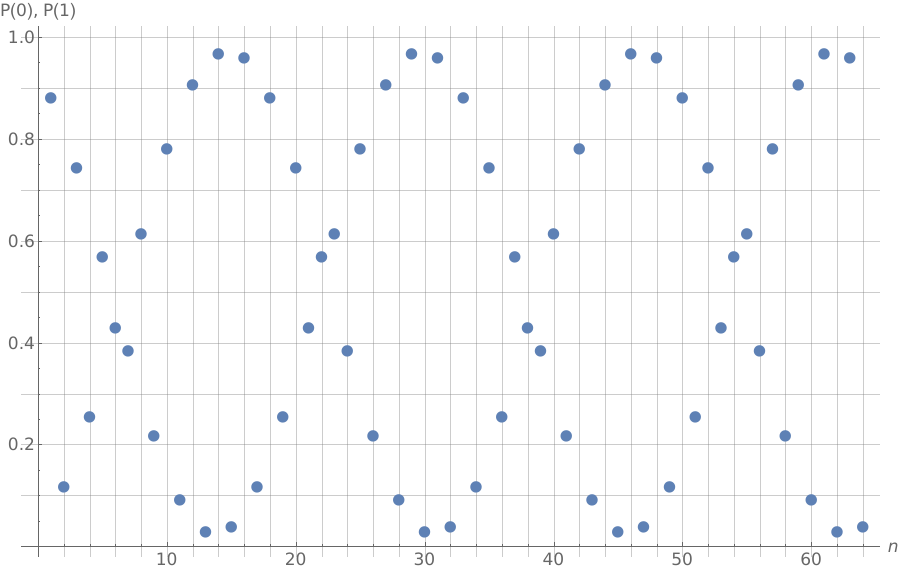
\includegraphics[height=.3\textheight]{img/N32-B.png}
  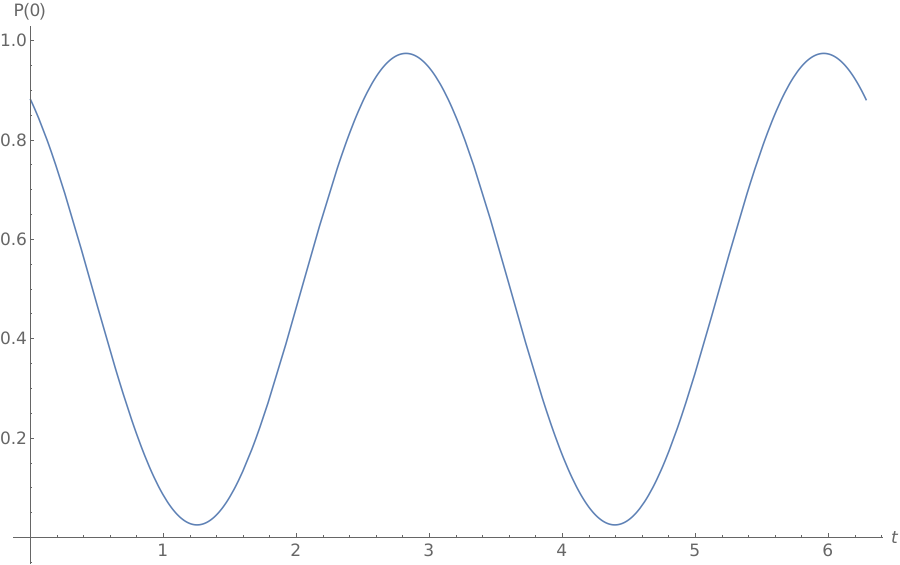
\includegraphics[height=.3\textheight]{img/probB_0.png}
  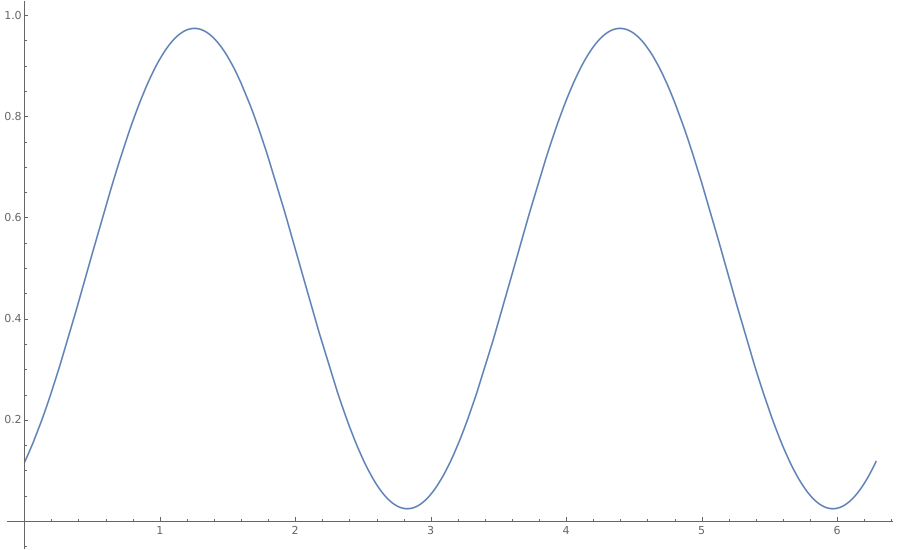
\includegraphics[height=.3\textheight]{img/probB_1.png}
  \caption[
    Page-Wootters vs Schr{\"o}dinger probability evolution
  ]{
    Page-Wootters ({\it top}) vs Schr{\"o}dinger probability evolution. % for $\op{\mathbb{J}}$ eigenvalue $=11$.
    See also Eqs. \eqref{eq:comparison0} and \eqref{eq:comparison0}.
  }
  \label{fig:prob-comparison}
\end{figure}

Figure \ref{fig:prob-comparison} is the graphical representation of (the square modulus of)
\eqref{eq:comparison0} and \eqref{eq:comparison1} i.e. the probability for the qubit
in $\hilb{H}_S$ to be $\ket{0}$ or $\ket{1}$.

The discrete graph, on top, plots the
square modulus of components of $\op{\mathbb{J}}$'s eigenvector $\dket{\Psi_{41}}$.

Odd-index ($2k+1$) square-modulus components
---occupying vertical \emph{spaces} on the grid---
are compared
with the Schr{\"o}dinger evolution of probability $\qty|\braket{0}{\psi}|^{2}$
(first continuous plot, middle image).

Even-index ($2k+2$) components
---occupying vertical \emph{lines} on the grid---
are analogously compared
with the Schr{\"o}dinger evolution of probability $\qty|\braket{1}{\psi}|^{2}$
(second continuous plot, bottom image).

\begin{figure}
  \centering
  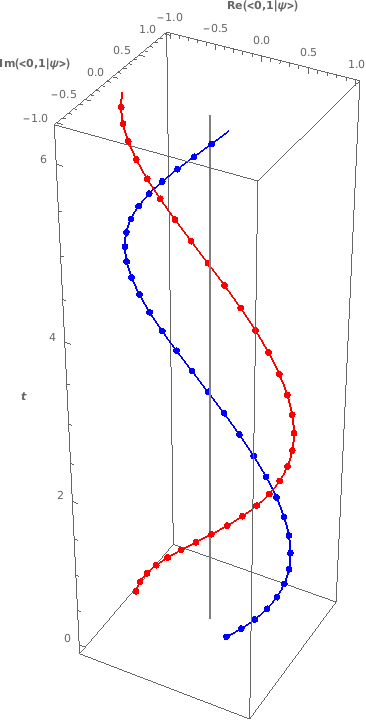
\includegraphics[width=0.45\textwidth]{img/PWfit32.png}
  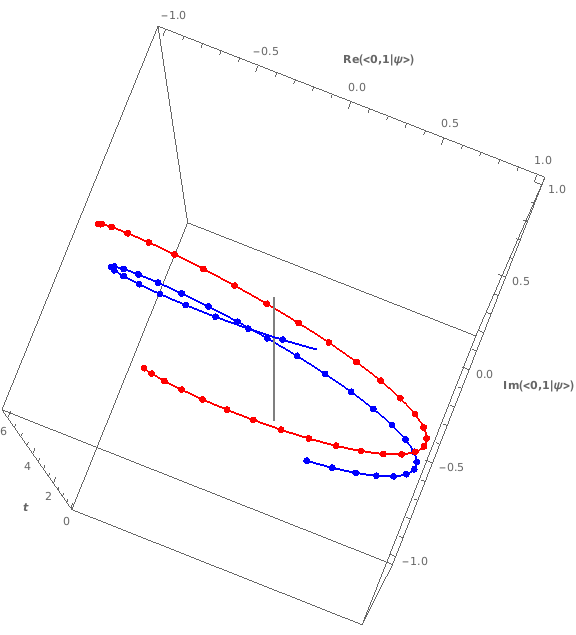
\includegraphics[width=0.5\textwidth]{img/PWfit32top.png}
  \caption[
    P-W vs Schr{\"o}dinger evolution (complex values)
  ]{
    Page--Wootters discrete-time ``evolution without evolution'' (points)
    is interpolated by the (continuous lines) of standard quantum mechanics
    evolution.
    Horizontal axis are real and imaginary part of the wave function components.
    Vertical axis is time $t$.
    Red   line plots {\color{red}   $\braket{0}{\psi(t)}$}.
    Blue  line plots {\color{blue}  $\braket{1}{\psi(t)}$}.
  }
  \label{fig:complex-comparison}
\end{figure}

Finally, Figure \ref{fig:complex-comparison} compares the two sides of
\eqref{eq:comparison0} and \eqref{eq:comparison1}
in terms of \emph{complex value}
(%
  therefore the term $e^{-i \epsilon t_k}$ is relevant,
  for eigenvalues $\epsilon \neq 0$ of $\op{\mathbb{J}}$%
).
